\lstset{language = c}
\section{OpenGL}
The program created for this part of the assignment, 
is made by modifying code given to us for the graphics part of the course. 
The color-buffers and the vertex-buffer is created in the initialization phase. 
For each frame drawn, RenderScene is called. Most of the important code is found inside that function.
The txt-file is read once for each object everytime RenderScene is called. This could perhaps have been more efficient. But as the program did not seem to slow down because of it, no changes where made.
The text-file is read using ReadFile.cpp.
ReadFile uses the windows library conio.h to read the file. 
The read function used to get the values, requires an integer representing a line in the .txt as input.
Parameters requiered to represent the object is extracted from that line, and placed in a array.
A pointer to the first parameter is then returned.
\\
By reading the txt-file each time the scene is rendered, the program is able to change the scene while running.
This is done by modifying the txt-file. 
Each cube needs four parameters to be represented.
One for color, one for radius, one for the x-coordinate and one for the y-coordinate. The format in the exchange file looks like this:
\\
\lstinputlisting[lastline=2]{../test.txt}
\mbox{}\\
The fist line represents a shape with the following parameters:
\\color: red(1), radius=11, coord-x=300, coord-y=76.
\\
After setting the values, a model-matrix for the shape is made. 
The model-matrix consists of an identity-matrix multiplyed with a translation-matrix, multiplyed with a scale-matrix. 
The model-matrix for the cube represents the radius and position of the object.
\lstinputlisting[firstline=337, lastline = 347]{../opengl/visuals.cpp} 
After multiplying the model-matrix with the mvp-matrix, a color-buffer and a vertex-buffer is bound before drawing the shape.
The process is repeated until all objects are represented. 
below is a screenshot taken from the program running.
\\
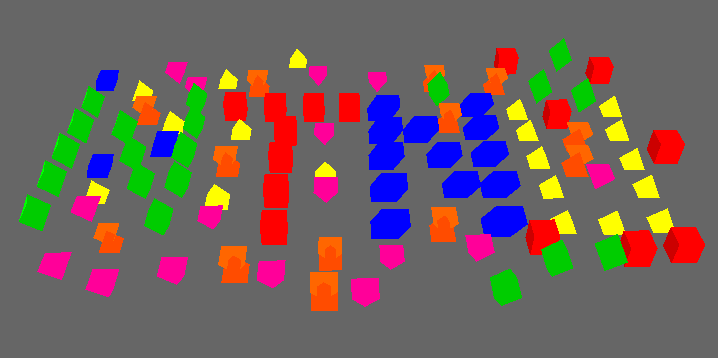
\includegraphics[scale=0.75]{Screen1.png}
\mbox{}\\
The shapes are counted once when the program starts. 
\lstinputlisting[firstline=751, lastline=783]{../opengl/visuals.cpp}
To display the numbers, a vertexbuffer is created for the numbers 0 to 9. To number-buffers are drawn when the shape is drawn. The highest number the program is able to display is 99. One mvp-matrix is created for each number. The rotation matrix rotates the number about the y-axis. The rotation speed is determined by a counter. 
\\
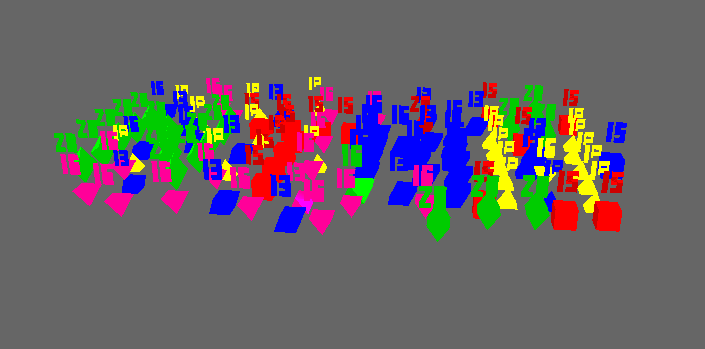
\includegraphics[scale=0.75]{with_numbers.png}
\mbox{}\\

\subsection{Improvements}
Today, the cubes are given color by static pre-made color-buffers. 
To support all colors, one buffer for each different color given in the input-file should be made. 
A solution like that was considered, but not pursued.
Lack of experience programming in the C-language, resulted in our program not being able to support dynamically made colorbuffers.
\\
The matrices could have been better structured using the joining techniques from lab4. However the requirement of having numbers where noticed late and other projects might have been prioriticed at this moment. 

